\documentclass[12pt,a4paper]{article}

\usepackage{tikz}\usetikzlibrary{automata,arrows,snakes,shapes}
\usepackage{amssymb}
\usepackage{amsmath}

\usepackage{ngerman}
\usepackage[latin1]{inputenc}
\usepackage[T1]{fontenc}
\usepackage{microtype}
\usepackage{fixltx2e}
%\usepackage{ifthen}
%\usepackage{fancyhdr}
\usepackage{booktabs}
\usepackage{xspace}

\DeclareMathOperator{\mask}{Mask}
\DeclareMathOperator{\fine}{fine}
\DeclareMathOperator{\coarse}{coarse}
\DeclareMathOperator{\vmod}{mod}

\newcommand{\fieldfine}{V_{\fine}}
\newcommand{\fieldcoarse}{V_{\coarse}}
\newcommand{\velmodel}{V_{\vmod}}

\newcommand{\maskfine}{\mask_{\fine}}
\newcommand{\maskcoarse}{\mask_{\coarse}}

\newcommand{\slantstacks}{D_S}
\newcommand{\outp}{O}
\newcommand{\updatedescr}{U}

\DeclareMathOperator{\oppartof}{PART}
\DeclareMathOperator{\opfull}{FULL}

\newcommand{\parens}[3]{#1#3#2}
\newcommand{\K}[1]{\parens{(}{)}{#1}}
\newcommand{\card}[1]{\parens{|}{|}{#1}}
\newcommand{\set}[1]{\parens{\{}{\}}{#1}}
\newcommand{\lst}[1]{\parens{[}{]}{#1}}
\newcommand{\scalar}[2]{\langle#1|#2\rangle}

\newcommand{\partof}[1]{\oppartof{}\K{#1}}
\newcommand{\full}[1]{\opfull{}\K{#1}}

\begin{document}

\title{UFBMig -- Ultra Fast Beam Migration}

\author{Mirko Rahn}

\maketitle

\subsection*{Data}

\begin{itemize}
\item velocity fields, fine, coarse + smooth:
  \begin{description}
  \item[$\fieldfine$] available via a file that is suitable for parallel
    access

    needed only during initialization to calculate $\fieldcoarse$

  \item[$\fieldcoarse$] calculated from $\fieldfine$

    distributed storage, each node holds a part
  \end{description}

\item salt mask, fine, coarse + smooth:
  \begin{description}
  \item[$\maskfine$] send by a single producer (typically the GUI)

    should be distributed across nodes

    needed only during calculation of $\maskcoarse$

  \item[$\maskcoarse$] calculated from $\maskfine$

    distributed storage, each node holds a part
  \end{description}

\item velocity model (spline coefficients):
  \begin{description}
  \item[$\velmodel$] calculated from $\fieldcoarse$ and $\maskcoarse$

      for minimal latency stored repeatedly, each node holds a
      complete copy
  \end{description}

\item slantstacks, the preprocessed input:
  \begin{description}
  \item[$\slantstacks$] available via a file that is suitable for
    parallel access

    splitable in chunks of any size
  \end{description}

\item output volume:
  \begin{description}
  \item[$\outp$] splitable in chunks of any size

    distributed storage

    should be either stored (in parallel) or send to a consumer
    (typically the GUI) by a single node
  \end{description}

\item update description:
  \begin{description}
  \item[$\updatedescr$] contains all updates for the complete output volume
  \end{description}

\end{itemize}

\subsection*{Algorithms}

\begin{itemize}
\item coarse \& smooth: $\fieldfine \to \fieldcoarse$
  \begin{itemize}
  \item parallel algorithm
  \item includes parallel load with overlap
  \item either maximal overlap or communication
  \item virtual memory:
    \begin{itemize}
    \item leaves $\partof{\fieldcoarse}$
    \end{itemize}
  \item working memory:
    \begin{itemize}
    \item buffers $\partof{\fieldfine}$, could be a mmap
    \item buffers $\partof{\fieldcoarse}$
    \end{itemize}
  \end{itemize}

\item coarse \& smooth: $\maskfine \to \maskcoarse$
  \begin{itemize}
  \item parallel algorithm
  \item no parallel load, instead distributed by a single node
  \item start one workflow per work package
  \item either maximal overlap or communication
  \item virtual memory:
    \begin{itemize}
    \item leaves $\partof{\maskcoarse}$
    \item buffers $\partof{\maskfine}$
    \end{itemize}
  \item working memory:
    \begin{itemize}
    \item buffers $\partof{\maskfine}$
    \item buffers $\partof{\maskcoarse}$
    \end{itemize}
  \end{itemize}

\item build model: $\fieldcoarse \to \maskcoarse \to \velmodel$
  \begin{itemize}
  \item each node does the same
  \item each node accesses $\full{\fieldcoarse}$ and $\full{\maskcoarse}$
  \item virtual memory:
    \begin{itemize}
    \item uses $\partof{\fieldcoarse}$
    \item uses $\partof{\maskcoarse}$
    \item buffers $\partof{\fieldcoarse}$
    \item buffers $\partof{\maskcoarse}$
    \end{itemize}
  \item working memory:
    \begin{itemize}
    \item buffers $\partof{\fieldcoarse}$
    \item buffers $\partof{\maskcoarse}$
    \item leaves $\full{\velmodel}$
    \end{itemize}
  \end{itemize}

\item calculate: $\slantstacks \to \velmodel \to \updatedescr$
  \begin{description}
  \item[Variant A] reads the input data from a cache in the virtual
    memory

    makes sense only when I/O and calculation can overlap

    makes sense only when the cache is kept warm after a complete
    calculation

  \item[Variant B] reads the input data directly from the disk into
    the working memory as needed

    avoids communication from/to virtual memory

    produces more I/O in case of repeated calculations

  \end{description}
  \begin{itemize}
  \item before doing the calculation, one has to check whether or not
    the $\velmodel$ is up to date. In case of an outdated $\velmodel$
    one has to start the model calculation
  \item virtual memory:
    \begin{itemize}
    \item leaves $\updatedescr$
    \item buffers $\partof{\slantstacks}$ (only in Variant A)
    \end{itemize}
  \item working memory:
    \begin{itemize}
    \item uses $\full{\velmodel}$
    \item buffers $\partof{\slantstacks}$
    \item buffers $\updatedescr$
    \end{itemize}
  \end{itemize}

\item split update: $\updatedescr \to \lst{\updatedescr}$
  \begin{itemize}
  \item virtual memory:
    \begin{itemize}
    \item updates $\updatedescr$ to $\lst{\updatedescr}$
    \end{itemize}
  \item working memory:
    \begin{itemize}
    \item buffers $\updatedescr$
    \item buffers $\lst{\updatedescr}$
    \end{itemize}
  \item heap memory:
    \begin{itemize}
    \item buffers $\updatedescr$
    \end{itemize}
  \end{itemize}

\item update: $\updatedescr \to \outp \to \outp$
  \begin{itemize}
  \item virtual memory:
    \begin{itemize}
    \item uses $\updatedescr$
    \item updates $\partof{\outp}$
    \end{itemize}
  \item working memory:
    \begin{itemize}
    \item buffers $\updatedescr$
    \item buffers $\partof{\outp}$
    \end{itemize}
  \end{itemize}

\end{itemize}

\subsection*{Usage}

The main usage scenario is a single init, follow by a number of
calculations for different salt masks.

\begin{center}
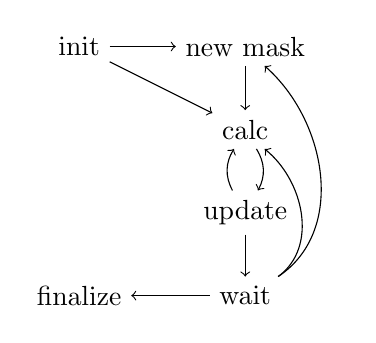
\begin{tikzpicture}
\tikzstyle{every node}+=[node distance=6em]

\node (init) {init};
\node (new_mask) [right of=init] {new mask};
\node (calc) [below of=new_mask,node distance=3em] {calc};
\node (update) [below of=calc,node distance=3em] {update};
\node (wait) [below of=update,node distance=3em] {wait};
\node (finalize) [left of=wait] {finalize};

\path[->]
  (init) edge (new_mask)
  (init) edge (calc)
  (new_mask) edge (calc)
  (calc) edge [bend left] (update)
  (update) edge [bend left] (calc)
  (update) edge (wait)
  (wait) edge (finalize)
  (wait) edge [bend right, out=300, in=225] (new_mask)
  (wait) edge [bend right, out=300, in=225] (calc)
;
\end{tikzpicture}
\end{center}

\subsection*{Memory Layout}

From the usage scenario we can derive the memory layout.

Right after the init, the $\fieldcoarse$ is stored in the virtual
memory. It has to be there all the time, since it is needed to
calculate the new velocity model (during calc).

We have to store the $\maskcoarse$ as well in virtual memory, since
the complete information is needed to calculate the velocity model
$\velmodel$. We could delete it from there after the calculation of
$\velmodel$, but this would require a parallel process which we do not
have at the moment.

The $\velmodel$ itself will be stored in the working memory of the
node. This is because of the access pattern: Many small fetches.

The update descriptions are communicated via the virtual memory as
well and the output volume is stored there.

So we have per node:
\begin{description}
\item[virtual memory]~

  \begin{itemize}
  \item $\partof{\fieldcoarse}$
  \item $\partof{\maskcoarse}$
  \item $\partof{\outp}$
  \item $\updatedescr$
  \end{itemize}
\item[working memory]~

  \begin{itemize}
  \item $\full{\velmodel}$
  \end{itemize}
\end{description}

Besides this, the different algorithms needs to buffer some
intermediate data, namely:

\begin{description}
\item[in virtual memory]~

  \begin{itemize}
  \item $\partof{\maskfine}$
  \end{itemize}
\item[in working memory]~

  \begin{itemize}
  \item $\partof{\maskfine}$
  \item $\partof{\maskcoarse}$
  \item $\partof{\slantstacks}$
  \item $\updatedescr$
  \item $\partof{\outp}$
  \end{itemize}
\end{description}


\subsection*{Setup}

We have a running SDPA system that is steered by a frontend. The
frontend sends commands, that is workflows to the SDPA
system. Commands are
\begin{itemize}
\item INIT, includes calculation of $\fieldcoarse$
\item NEW MASK, send a new salt mask, triggers calculation of
  $\maskcoarse$
\item CALCULATE, triggers calculation of $\velmodel$ if needed
\item DUMP, sends the result to a file or a socket or ...
\item FINALIZE, frees all resources
\item CANCEL
\end{itemize}

The very basic implementation of this frontend is just a collection of
the corresponding workflows.

The GUI will not communicate with this frontend directly but instead
with a backend, that itself will communicate with the frontend.

\begin{center}
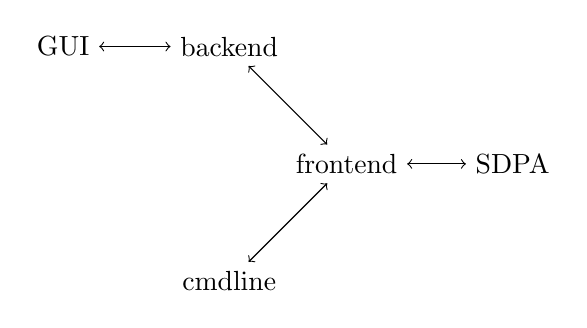
\begin{tikzpicture}
\tikzstyle{every node}+=[node distance=6em]
\node (sdpa) {SDPA};
\node (frontend) [left of=sdpa] {frontend};
\node (backend) [above left of=frontend] {backend};
\node (cmdline) [below left of=frontend] {cmdline};
\node (gui) [left of=backend] {GUI};

\path[<->]
  (sdpa) edge (frontend)
  (frontend) edge (backend)
  (cmdline) edge (frontend)
  (gui) edge (backend)
;
\end{tikzpicture}
\end{center}


\end{document}
